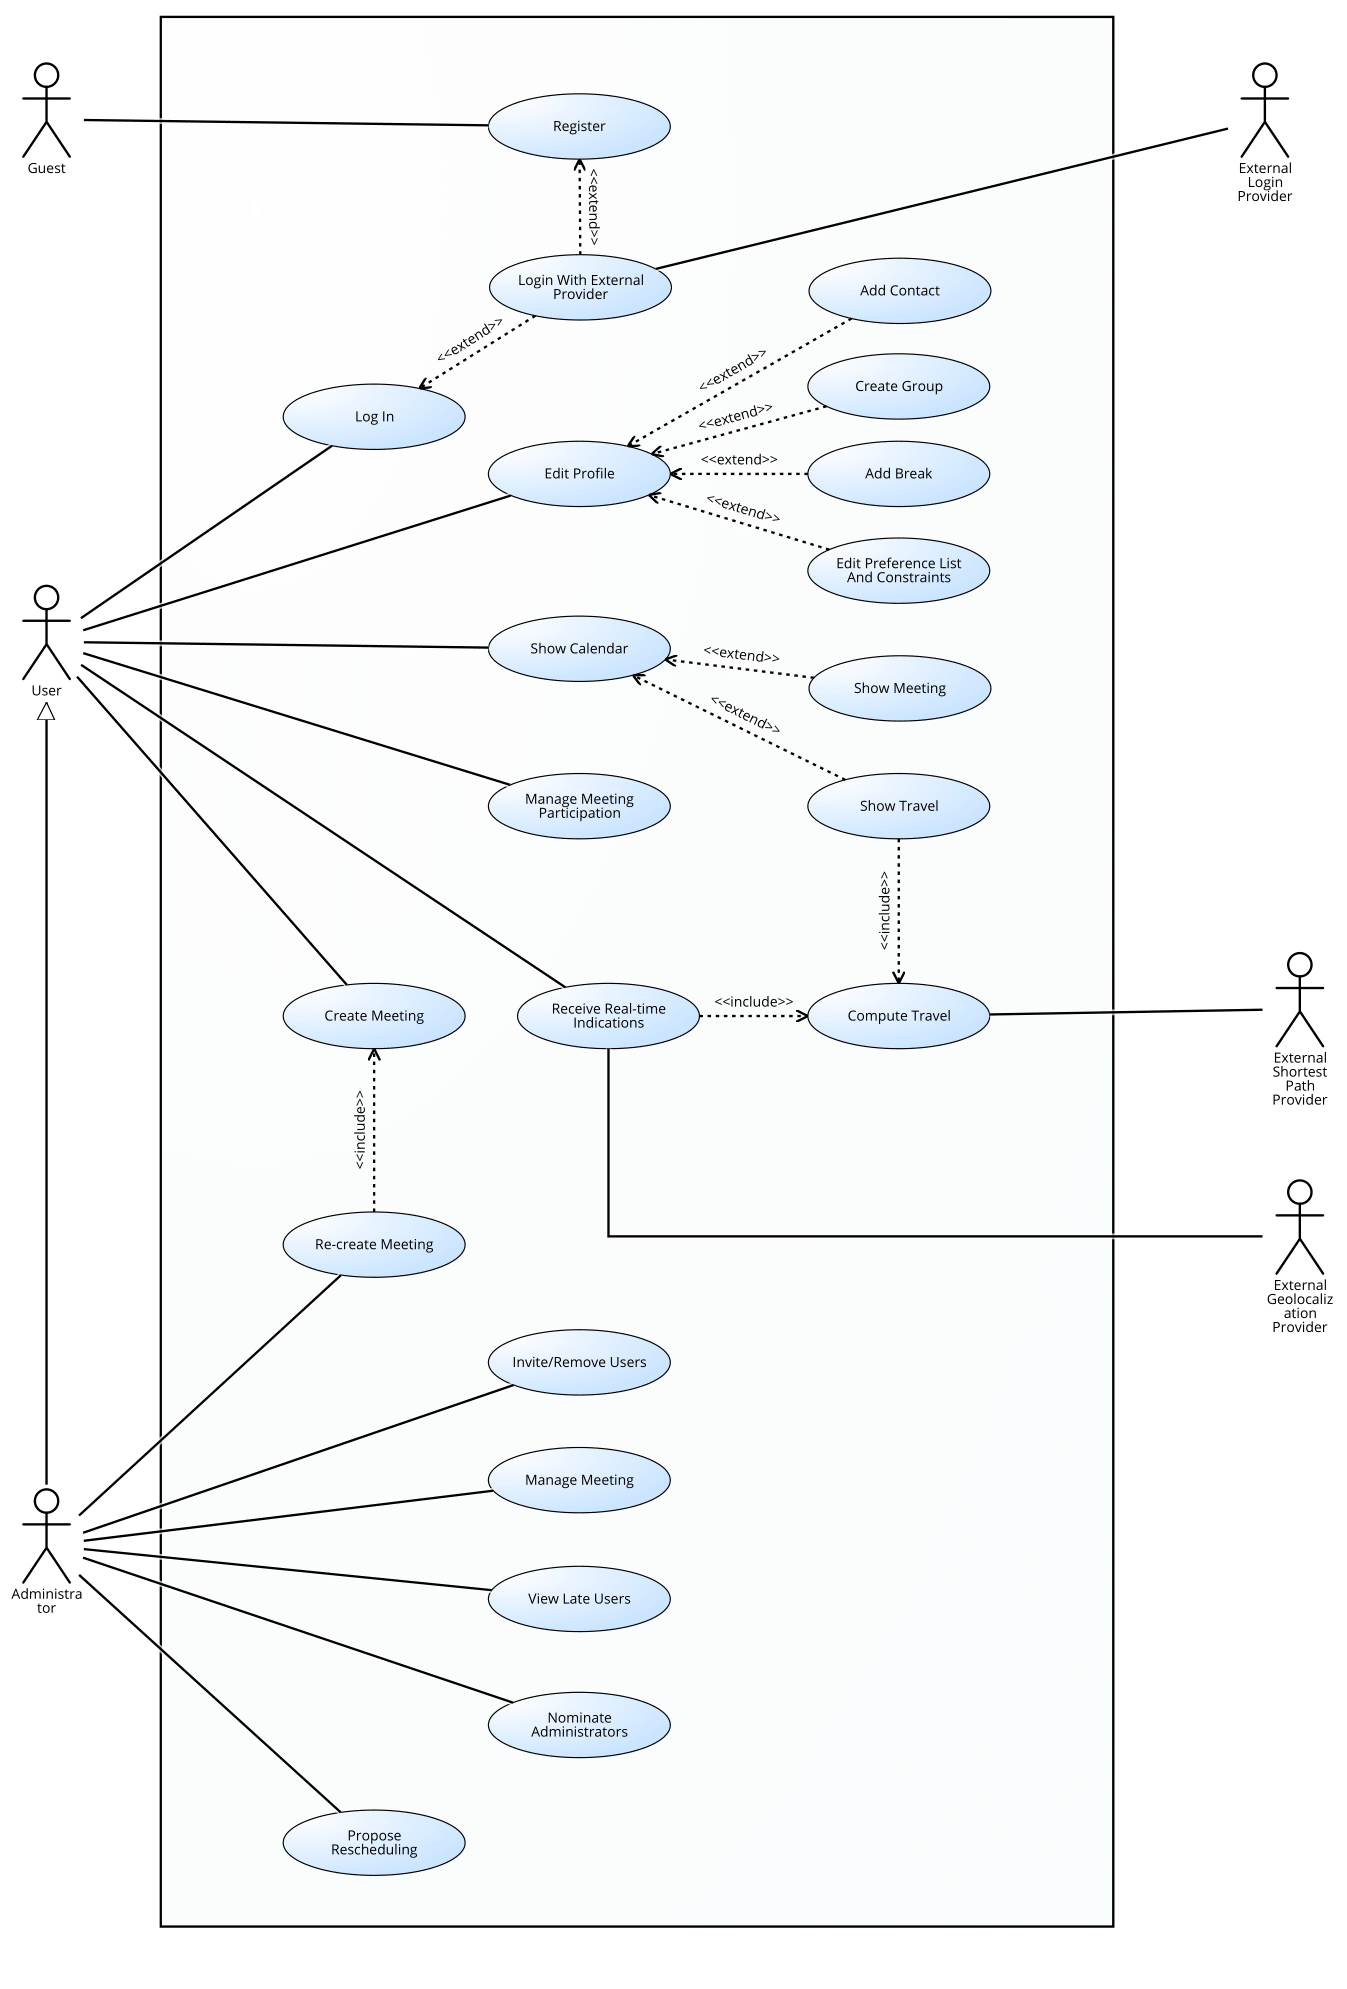
\includegraphics[height=\textheight, width=\textwidth]{Images/UseCaseDiagram.png}

\begin{table}[h]	
	\centering
	\def\arraystretch{1.5}
	\begin{tabular}{|m{7cm}|m{7cm}|}
		\hline
		\textbf{Actors}            & Guest, External Login Provider		    \\ \hline
		\textbf{Goals}             & \ref{goal:Registration}           \\ \hline
		\textbf{Input Conditions}  & A guest is on the homepage of the system.           \\ \hline
		\textbf{Events Flow}       &   
		\begin{enumerate}
			\item The guest inserts its main emailaddress.
			\item The guest enters its password.
			\item The guest clicks on the "Sign Up" button.
		\end{enumerate}    \\ \hline
		\textbf{Output Conditions} & The guest is registered into the system with a pair <email, password>. The guest is redirected to a page where it can add to its profile the compulsory information needed to use the system, that are: the preference list, a unique nickname and at least one default location.      \\ \hline
		\textbf{Exceptions}        & The guest inserts a wrong or already-used email. In this case the system shows the user a message reporting the errors and waits for another attempt.            \\ \hline
	\end{tabular}
	\caption[Registration]{{Registration}\label{UseCaseDescr:Registration} (view \hyperref[SeqDiagr:Registration]{Sequence Diagram})}
\end{table}

\begin{table}[h]
	\centering
	\def\arraystretch{1.5}
	\begin{tabular}{|m{7cm}|m{7cm}|}
		\hline
		\textbf{Actors}            & User, External Login Provider		    \\ \hline
		\textbf{Goals}             & \ref{goal:Login}           \\ \hline
		\textbf{Input Conditions}  & User is on the homepage of the system and it has not yet been authenticated.           \\ \hline
		\textbf{Events Flow}       &    
		\begin{enumerate}
			\item The user clicks on the "Log in with \texttt{Service name}" button.
			\item The user is taken to an external page where it has to follow the authentication procedure of the external login provider.
			\item The user is redirected to our system with a valid token.
		\end{enumerate} \\ \hline
		\textbf{Output Conditions} & User is logged into the system.          \\ \hline
		\textbf{Exceptions}        & The external login provider procedure cannot be completed correctly. In this case the system shows the user a message reporting the error.         \\ \hline
	\end{tabular}
	\caption[Login with External Provider]{{Login with External Provider}\label{UseCaseDescr:LoginExternal} (view \hyperref[SeqDiagr:LoginExternal]{Sequence Diagram})}
\end{table}

\begin{table}[h]
	\centering
	\def\arraystretch{1.5}
	\begin{tabular}{|m{7cm}|m{7cm}|}
		\hline
		\textbf{Actors}            & User	    \\ \hline
		\textbf{Goals}             & \ref{goal:Login}           \\ \hline
		\textbf{Input Conditions}  & User is on the homepage of the system and it has not yet been authenticated.           \\ \hline
		\textbf{Events Flow}       &    
			 	\begin{enumerate}
			 		\item The user inserts its main email address or its nickname.
			 		\item The user inserts its password.
			 		\item The user clicks on the "Log in" button.
			 	\end{enumerate}\\ \hline
		\textbf{Output Conditions} & User is logged into the system.          \\ \hline
		\textbf{Exceptions}        & The user credentials are wrong. The system shows the user a message reporting the errors and waits for another attempt.         \\ \hline
	\end{tabular}
	\caption[Login]{{Login}\label{UseCaseDescr:LoginNormal} (view \hyperref[SeqDiagr:LoginNormal]{Sequence Diagram})}
\end{table}

\begin{table}[h]
	\centering
	\def\arraystretch{1.5}
	\begin{tabular}{|m{7cm}|m{7cm}|}
		\hline
		\textbf{Actors}            & User		    \\ \hline
		\textbf{Goals}             & \ref{goal:EditProfile}          \\ \hline
		\textbf{Input Conditions}  & The user has already been authenticated by the system.           \\ \hline
		\textbf{Events Flow}       & 
			\begin{enumerate}[topsep=0pt, leftmargin=*]
				\item The user clicks on the "Edit" button on its profile page.
				\item The user selects a field to edit.
				\item The user inserts new data for the selected field.
				\item The user can repeat from point 2 or click the "Save" button.
				\item The system redirects the user to its profile page.
			\end{enumerate}           \\ \hline
		\textbf{Output Conditions} & The selected fields are updated with the new data inserted by the user.          \\ \hline
		\textbf{Exceptions}        &  The data inserted in a field are wrong (e.g. a non-unique nickname, a non-unique email, a syntactically wrong website, etc.). The system shows the user a message reporting the errors, clears the incorrect fields and restarts the event flow from point 2.               \\ \hline
	\end{tabular}
	\caption[Edit Profile]{{Edit Profile}\label{UseCaseDescr:EditProfile} (view \hyperref[SeqDiagr:EditProfile]{Sequence Diagram})}
\end{table}

\begin{table}[h]
	\centering
	\def\arraystretch{1.5}
	\begin{tabular}{|m{7cm}|m{7cm}|}
		\hline
		\textbf{Actors}            & User		    \\ \hline
		\textbf{Goals}             & \ref{goal:SeeSchedule}           \\ \hline
		\textbf{Input Conditions}  & The user has already been authenticated by the system.           \\ \hline
		\textbf{Events Flow}       & 
			\begin{enumerate}[topsep=0pt, leftmargin=*]
				\item The user clicks on the "Calendar" button in the menu.
				\item The system generates a page containing all the meetings and the travels of the day.
				\item The user may navigate to a week view and to a month view.
				\item The user may click on a meeting or on a travel to see it in detail.
			\end{enumerate}	           \\ \hline
		\textbf{Output Conditions} & This use case does not modify anything, so the state of the output is equal to the state of the input.           \\ \hline
		\textbf{Exceptions}        & There are no exceptions.           \\ \hline
	\end{tabular}
	\caption[Show Calendar]{{Show Calendar}\label{UseCaseDescr:ShowCalendar} (view \hyperref[SeqDiagr:ShowCalendar]{Sequence Diagram})}
\end{table}

\begin{table}[h]
	\centering
	\def\arraystretch{1.5}
	\begin{tabular}{|m{7cm}|m{7cm}|}
		\hline
		\textbf{Actors}            & User		    \\ \hline
		\textbf{Goals}             & \ref{goal:MeetingParticipation}           \\ \hline
		\textbf{Input Conditions}  & The user has already been authenticated by the system and has been invited to attend a meeting.           \\ \hline
		\textbf{Events Flow}       & 
			\begin{enumerate}[topsep=0pt, leftmargin=*]
				\item The user selects a meeting it wants to manage by clicking on it in the "Calendar" page.
				\item The system displays all the information about the selected meeting, such as the title, the date, the location and the other invited users.
				\item The user clicks on the "Accept", "Decline" or "Reschedule" button.
				\item In the latter case, the user selects a new proposed start date.
			\end{enumerate}           \\ \hline
		\textbf{Output Conditions} & The acceptance, refusal or rescheduling proposal of the meeting is recorded by the system. In the latter case, it is forwarded to the meeting administrator.           \\ \hline
		\textbf{Exceptions}        & The user selects an invalid start date (e.g. a date which is in the past). The system shows the user a message reporting the errors and wait for a new date to be inserted.           \\ \hline
	\end{tabular}
	\caption[Manage Meeting Participation]{{Manage Meeting Participation}\label{UseCaseDescr:MeetingPart} (view \hyperref[SeqDiagr:MeetingPart]{Sequence Diagram})}
\end{table}

\begin{table}[h]
	\centering
	\def\arraystretch{1.5}
	\begin{tabular}{|m{7cm}|m{7cm}|}
		\hline
		\textbf{Actors}            & User, External Geolocalization Provider, External Shortest Path Provider		    \\ \hline
		\textbf{Goals}             & \ref{goal:Travel}         \\ \hline
		\textbf{Input Conditions}  & The user has already been authenticated by the system and the system has detected that the start time of one of its meeting is approaching.           \\ \hline
		\textbf{Events Flow}       & 
			\begin{enumerate}[topsep=0pt, leftmargin=*]
				\item The system notifies the user that it's time for him to leave.
				\item By using the real-time position of the user, the system keeps giving him indications on where to go and what travel means to use.
				\item The user can click on the "Stop Notifications" button to stop the system giving him travel indications.
			\end{enumerate}	        \\ \hline
		\textbf{Output Conditions} & The user has reached the meeting location or the user has clicked the "Stop Notifications" button.           \\ \hline
		\textbf{Exceptions}        & There are no exceptions.           \\ \hline
	\end{tabular}
	\caption[Receive Real-Time Indications]{{Receive Real-Time Indications}\label{UseCaseDescr:RealTimeInd} (view \hyperref[SeqDiagr:RealTimeInd]{Receive Real-Sequence Diagram})}
\end{table}

\begin{table}[h]
	\centering
	\def\arraystretch{1.5}
	\begin{tabular}{|m{7cm}|m{7cm}|}
		\hline
		\textbf{Actors}            & User		    \\ \hline
		\textbf{Goals}             & \ref{goal:ManageMeeting}           \\ \hline
		\textbf{Input Conditions}  & The user has already been authenticated by the system.           \\ \hline
		\textbf{Events Flow}       & 
			\begin{enumerate}[topsep=0pt, leftmargin=*]
				\item The use clicks on the "Create Meeting" button.
				\item The user inserts a start date, an end date, a title and a location for the meeting.
				\item The user may add other data, such as an abstract or a category.
				\item The user chooses a non-empty list of invited users, either by inserting their email or by selecting them from its contacts; in alternative the user may specify that it is an instant meeting.
				\item The user clicks on the "Create" button.
				\item The system redirects the user to the new meeting page.
			\end{enumerate}               \\ \hline
		\textbf{Output Conditions} & A new meeting is created and an invitation is sent to all the selected users.           \\ \hline
		\textbf{Exceptions}        & The location of the meeting may be incorrect or the start and end date may be inconsistent (i.e. the start is after the end). The system shows the user a message reporting the errors, clears the incorrect fields and restart the event flow from point 2.          \\ \hline
	\end{tabular}
	\caption[Create Meeting]{{Create Meeting}\label{UseCaseDescr:CreateMeeting} (view \hyperref[SeqDiagr:CreateMeeting]{Sequence Diagram})}
\end{table}

\begin{table}[h]
	\centering
	\def\arraystretch{1.5}
	\begin{tabular}{|m{7cm}|m{7cm}|}
		\hline
		\textbf{Actors}            & Administrator    \\ \hline
		\textbf{Goals}             & \ref{goal:RecreateMeeting}           \\ \hline
		\textbf{Input Conditions}  & A meeting has been created and completed normally. The team decides that another meeting is necessary to fulfill their goals. \\ \hline
		\textbf{Events Flow}       & 
		\begin{enumerate}[topsep=0pt, leftmargin=*]
			\item One of the administrators clicks on the "Recreate Meeting" button.
			\item The system shows a meeting creation form where title, abstract, uploaded file and participants fields are pre-filled with the previous meeting's values.
			\item The administrator chooses the location and the date for the new meeting.
			\item The administrator clicks on the "Create" button.
		\end{enumerate}              \\ \hline
		\textbf{Output Conditions} & A new meeting is created and an invitation is sent to all the selected users.           \\ \hline
		\textbf{Exceptions}        & The location of the meeting may be incorrect or the start and end date may be inconsistent (i.e. the start is after the end). The system shows the user a message reporting the errors, clears the incorrect fields and restart the event
		flow from point 2.           \\ \hline
	\end{tabular}
	\caption[Recreate Meeting]{{Recreate Meeting}\label{UseCaseDescr:RecreateMeeting} (view \hyperref[SeqDiagr:RecreateMeeting]{Sequence Diagram})}
\end{table}

\begin{table}[h]
	\centering
	\def\arraystretch{1.5}
	\begin{tabular}{|m{7cm}|m{7cm}|}
		\hline
		\textbf{Actors}            & Administrator    \\ \hline
		\textbf{Goals}             & \ref{goal:InviteUsers}           \\ \hline
		\textbf{Input Conditions}  & A meeting has been created.           \\ \hline
		\textbf{Events Flow}       &  
		\begin{enumerate}[topsep=0pt, leftmargin=*]
			\item One of the administrators clicks on the "Add Participants" button on the meeting page.
			\item The administrator selects some users either by choosing from its contacts or by inserting their nickname or email.
			\item The Administrator clicks on the "Send" button to send invitations.
		\end{enumerate}           \\ \hline
		\textbf{Output Conditions} & The selected users receive meeting invitations.            \\ \hline
		\textbf{Exceptions}        & 
		The administrator may have write a wrong or non-existent email or nickname. The system shows the administrator a message reporting the errors, clears the incorrect fields and restarts the event flow from point 2.     \\ \hline
	\end{tabular}
	\caption[Invite Users]{{Invite Users}\label{UseCaseDescr:InviteUsers} (view \hyperref[SeqDiagr:InviteUsers]{Sequence Diagram})}
\end{table}

\begin{table}[h]
	\centering
	\def\arraystretch{1.5}
	\begin{tabular}{|m{7cm}|m{7cm}|}
		\hline
		\textbf{Actors}            & Administrator    \\ \hline
		\textbf{Goals}             & \ref{goal:InviteUsers}           \\ \hline
		\textbf{Input Conditions}  & A meeting has been created.           \\ \hline
		\textbf{Events Flow}       & 
		\begin{enumerate}[topsep=0pt, leftmargin=*]
			\item One of the administrator clicks on the "Show Participants" button on the meeting page.
			\item The system shows the list of all users that have been invited to the meeting.
			\item The administrator can remove users from the participants list by clicking on the "Delete" button next to their name.
		\end{enumerate}            \\ \hline
		\textbf{Output Conditions} & The selected users are removed from the team.            \\ \hline
		\textbf{Exceptions}        & 
		There are no exceptions.         \\ \hline
	\end{tabular}
	\caption[Remove Users]{{Remove Users}\label{UseCaseDescr:RemoveUsers} (view \hyperref[SeqDiagr:RemoveUsers]{Sequence Diagram})}
\end{table}

\begin{table}[h]
	\centering
	\def\arraystretch{1.5}
	\begin{tabular}{|m{7cm}|m{7cm}|}
		\hline
		\textbf{Actors}            & Administrator    \\ \hline
		\textbf{Goals}             & \ref{goal:ViewLateUsers}           \\ \hline
		\textbf{Input Conditions}  & A meeting has been created and its start time has passed.         \\ \hline
		\textbf{Events Flow}       &  
		\begin{enumerate}[topsep=0pt, leftmargin=*]
			\item One of the administrator clicks on the "Who's Late" button on the meeting page.
			\item The administrator can contact one of the late participant clicking on his name.
		\end{enumerate}             \\ \hline
		\textbf{Output Conditions} & The administrator knows who is late and can take decisions based on that.           \\ \hline
		\textbf{Exceptions}        & There are no exceptions.           \\ \hline
	\end{tabular}
	\caption[View Late Users]{{View Late Users}\label{UseCaseDescr:LateUsers} (view \hyperref[SeqDiagr:LateUsers]{Sequence Diagram})}
\end{table}

\begin{table}[h]
	\centering
	\def\arraystretch{1.5}
	\begin{tabular}{|m{7cm}|m{7cm}|}
		\hline
		\textbf{Actors}            & Administrator    \\ \hline
		\textbf{Goals}             & \ref{goal:NominateAdmin}           \\ \hline
		\textbf{Input Conditions}  & A meeting has been created.           \\ \hline
		\textbf{Events Flow}       &  
		\begin{enumerate}[topsep=0pt, leftmargin=*]
			\item One of the administrator clicks on the "Show Participants" button.
			\item The system shows the list of all the users who have been invited to the meeting, with a "Nominate" button available only next to those who has accepted the invitation.
			\item The administrator clicks on the "Nominate" button next to users who wants to nominate administrator.
		\end{enumerate}             \\ \hline
		\textbf{Output Conditions} & Selected users become administrators and gain all the functionalities of the role.           \\ \hline
		\textbf{Exceptions}        & A participant may have decided to leave the meeting while the administrator's "Show Participant" page is open. In this case, if the participant is selected to be nominated as administrator, the system signals it with a message saying "this participant has left the meeting".      \\ \hline
	\end{tabular}
	\caption[Nominate Administrators]{{Nominate Administrators}\label{UseCaseDescr:NominateAdmin} (view \hyperref[SeqDiagr:NominateAdmin]{Sequence Diagram})}
\end{table}


\begin{table}[h]
\centering
\def\arraystretch{1.5}
\begin{tabular}{|m{7cm}|m{7cm}|}
	\hline
	\textbf{Actors}            & Administrator    \\ \hline
	\textbf{Goals}             & \ref{goal:EditMeeting}\newline \ref{goal:ShareFiles}           \\ \hline
	\textbf{Input Conditions}  & A meeting has been created.           \\ \hline
	\textbf{Events Flow}       &  
	\begin{enumerate}[topsep=0pt, leftmargin=*]
		\item One of the administrators clicks on the "Meeting Settings" button.
		\item The system shows all the functionalities available, such as edit title, modify abstract or upload files.
		\item The administrator can update all the fields.
		\item The administrator may chose to upload a file, to share it with the team, by clicking on the "Upload File" button.
		\item The administrator selects the file he wants to upload.
		\item The administrator clicks on the "Save" button.
	\end{enumerate}             \\ \hline
	\textbf{Output Conditions} & The fields are updated and the selected files are uploaded.          \\ \hline
	\textbf{Exceptions}        & The administrator wants  to upload a huge file or a file with an invalid extension. In this case, the system stops the upload of the file and shows the user a message saying "The file is not supported". \\ \hline
\end{tabular}
\caption[Manage Meeting]{{Manage Meeting}\label{UseCaseDescr:ManageMeeting} (view \hyperref[SeqDiagr:ManageMeeting]{Sequence Diagram})}
\end{table}

\begin{table}[h]
	\centering
	\def\arraystretch{1.5}
	\begin{tabular}{|m{7cm}|m{7cm}|}
		\hline
		\textbf{Actors}           & Administrator    \\ \hline
		\textbf{Goals}            & \ref{goal:RescheduleFromUser} \newline \ref{goal:RescheduleFromAdmin}           \\ \hline
		{\textbf{Input Conditions}}  & A meeting has been created.           \\ \hline
		{\textbf{Events Flow}}       &
		\begin{enumerate}[topsep=0pt, leftmargin=*]					
			\item One of the administrators clicks on the "Send Reschedule Proposal" button on the meeting page or on the reschedule proposal sent by an invited user.
			\item The system shows the reschedule form, pre-filled with the reschedule proposal data if the request comes from a user.
			\item The administrator completes the form.
			\item The administrator clicks on the "Send" button.
		\end{enumerate}                         \\ \hline
		\textbf{Output Conditions} & A rescheduling proposal is sent to all the participants. If everyone accepts than the meeting's date is changed.         \\ \hline
		\textbf{Exceptions}        & The inserted date is incorrect (e.g. in the past) or it does not differ from the previous one. The system shows a message reporting the errors, clears the incorrect fields and restarts the event flow from point 3.  \\ \hline
	\end{tabular}
	\caption[Propose Rescheduling]{{Propose Rescheduling}\label{UseCaseDescr:ProposeRes} (view \hyperref[SeqDiagr:ProposeRes]{Sequence Diagram})}
\end{table}

\clearpage
\newpage